
\begin{document}
\pagestyle{empty}
\chapter{Mutational signatures in \textit{C. elegans}}

\section{Introduction}

\todo[inline]{transition from the introduction of the screen to here}

In this chapter, I will describe the quantitative characteristics and
prospective mechanistic insights of the mutations introduces by DNA 
repair deficiencies in \textit{C. elegans} genome.

%%%%%%%%%%%%%%%%%%%%%%%%%%%%%%%%%%%%%%%%%%%%%%%%%%%%%%%%%%%%%%%%%%%%%%%%%%%%%%%%%%%%%%%%%%%%%%%%%%%

\subsection*{Contributions}

\todo[inline]{describe mine and bettina's contributions: visualisation and stats and stratifiction vs microhomology and mechanisms}

%%%%%%%%%%%%%%%%%%%%%%%%%%%%%%%%%%%%%%%%%%%%%%%%%%%%%%%%%%%%%%%%%%%%%%%%%%%%%%%%%%%%%%%%%%%%%%%%%%%

\section{Patterns of mutations generated under DNA repair deficiencies}

Signatures extracted for different genetic conditions also mostly coincide with 
the expected effects based on the function of the genes (\cite{p53}, \cite{Meier1},
\cite{DNArepair}, \cite{DNAdamagerepair}). In the examples in the Figure N the 
following effects are presented: impact of ageing, \textit{brc-1} - BRCA1 ortholog 
encoding gene which contributes to homologous recombination, \textit{cep-1} - 
P53-like protein encoding gene which regulated damage-caused cell apoptosis, 
and \textit{smg-1} - kinase-related protein kinase SMG1 which regulates oxidative stress response.

\subsection{Estimating mutation rates}

Accumulation of mutations was achieved through passing the \textit{C. elegans} 
lines through several generations, introducing a single-cell bottleneck at each 
generation passage. We assume that all mutations accumulated in a single cell 
are heterozygous; they have 25\% chance of being lost after propagation, 50\% 
chance of remaining heterozygous, and 25\% change of being fixed (becoming homozygous). 
Hence, in order to make the number of mutations directly proportional to the number of 
generations, we adjusted number of generations as

\[\tilde{N} = \lambda(N) = \sum_{i=1}^{N} \frac{1}{2^{i-1}} + \frac{1}{4} \sum_{i=1}^{N-1} \sum_{j=1}^{i} \frac{1}{2^{j-1}},\]

were $\tilde{N}$ denotes the adjusted generation number and $\lambda$ is a 
function reflecting the fraction of all accumulated mutations observed after $N$ generations.


\subsubsection*{Mutational signatures in mutations per generation}

\textit{rev-1} gene encodes an ortholog of human translesion polymerase REV1 which 
helps polymerases epsilon and delta to overcome stalled replication fork by inserting 
cytosins at abasic sites. As shown in Figure N, knocking out this gene does not 
significantly affect the mutational spectra in mutation accumulation experiment, 
but remarkably expands the mutational effects of DMS, which normally produces 
base substitutions and frameshift mutations and deletions.

\textit{xpa-1} encodes an ortholog of the human zinc finger protein XPA involved in nucleotide excision repair, which does not produce mutations when knocked-out alone, but expands the substitution mutational effects of alkylating agents and Gamma-irradiation, as shown in Figure N.


\subsection{Genetic interactions}

Apart from quantifying per-generation mutation rates for various knock-outs 
and effects of mutagen exposure, we have also identified several significant 
interaction effects, the underlying biology of which needs further investigation.

One example of a significant interaction between genetic backgrounds is the 
epistatic effect observed between mismatch repair system components \textit{pms-2} 
and \textit{pole-4}. \textit{pms-2} is a component of mismatch repair complex 
formed by attachment to \textit{mlh-1}. Both of these genes produce similar 
remarkable effects spectra when knocked-out, which agrees with the underlying biology 
(\cite{Denver2005-jh}).

\textit{pole-4} is a catalytic subunit 4 of the ortholog of human polymerase epsilon, 
which is assumed to have mostly repair function correcting the errors made by polymerase 
delta. When knocked out on its own, this gene does not cause significant changes in 
the samples, but the double mutants with both defective \textit{pms-2} and defective 
\textit{pole-4} show a 3-fold increase in the overall mutation amount. Deficiencies 
in human polymerase epsilon and polymerase delta were previously reported as driver 
genes in hypermutated brain cancers (\cite{Shlien2015-vw}).

The \textit{C. elegans} genome does not encode obvious MutL $\beta$ and $\gamma$ subunits 
(PMS1 and MLH3 homologues, respectively), while the MutL $\alpha$ subunits MLH1 and PMS2 
can be readily identified using homology searches. Given that null alleles of the human 
and \textit{C. elegans} leading strand polymerase pol-$\epsilon$ catalytic subunit, 
POLE and pole-1, respectively, are essential for viability, we focused our analysis 
on a non-essential \textit{C. elegans} pol-$\epsilon$ subunit, termed POLE-4. Dbp3p, 
the \textit{S. cerevisiae} POLE-4 ortholog, has been implicated in the stabilization 
of POLE with the primer-template DNA complex (\cite{Aksenova2010-rt}).

We detected an average of 4 base substitutions and 2 insertions or deletions in 
wild-type C. elegans lines propagated for 20 generations (**FIG**). In contrast, 
\textit{mlh-1} and \textit{pms-2} mutants carried an average of 1174 and 1191 unique mutations, 
respectively, of which 288 and 309 were base substitutions (**FIG**) and 886 
and 882 indels, defined as small insertions and deletions of less than 100 
base pairs (**FIG**). We did not find any structural variants (SVs) in all 
genotypes analyzed except for the pole-4 mutant, where one SV was observed 
in three mutation accumulation lines (**FIG**). The nature 
of single nucleotide changes and the overall mutation burden were congruent 
across independent lines of the same genotype and mutation numbers linearly 
increased from F10 to F20 generation lines (**FIG**). Thus, despite 
the high mutation frequency observed in MMR mutants, we did not observe 
evidence for secondary mutations that altered mutation profiles or frequencies. 
In contrast to \textit{mlh-1} and \textit{pms-2} mutants, \textit{pole-4} lines exhibited mutation rates 
and profiles not significantly different from wild-type (**FIG**) a 
finding we confirmed for \textit{pole-4} lines propagated over 40 generations (**FIG**).


\textbf{Mutation rates and patterns in \textit{pole-4; pms-2} double mutants}

To further investigate the role of pole-4 and the genetic interaction with 
MMR deficiency, we generated pole-4; pms-2 double mutants. Wild-type, pms-2, 
pole-4 and pole-4; pms-2 strains obtained as siblings from a cross of highly 
backcrossed pms-2 and pole-4 single mutants were grown for 10 generations and 
analyzed for mutation frequency and profiles. pms-2 mutant strains carried an 
average of 145 base substitution and 527 indels over 10 generations, roughly 
half the number we observed in the F20 generation (Fig. 1C and 1D, Table 2). 
In comparison, the number of single base substitutions and indels was increased 
~4.4 fold and ~1.4 fold in pole-4; pms-2 double mutants to an average of 637 and 723, 
respectively (Table 2, Figures 1C, 1D). No increased frequency of structural 
variants and chromosomal rearrangements was observed in pms-2 single or pole-4; pms 2 
double mutants (Table 2). We could not readily propagate pole-4; pms-2 beyond the 
F10 generation, suggesting that a mutation burden higher than ~500-700 single base 
substitutions (Fig. 1C) in conjunction with the 700-800 indels (Fig. 1D) might be 
incompatible with organismal reproduction. These numbers are in line with us not 
being able to stably propagate mlh-1 and pms-2 single mutant lines for 40 generations. 
The multiplicative effect on mutation burden detected in pole-4; pms-2 double mutants 
while no increased mutation rate is observed in pole-4 alone suggests that replication 
errors occur at increased frequency in the absence of C. elegans pole-4 but are 
effectively repaired by MMR.


Given the C. elegans genome size of 100 million base pairs, assuming that it 
takes 15 cell divisions to go through the C. elegans life cycle, and taking 
into account that heterozygous mutations can be lost during self-fertilization, 
we estimated the overall mutation rate for wild-type of 1.0 x 10-9  
(95\% CI: 7.96 x 10-10 to 1.25 x 10-9) per base pair and germ cell division 
and of 1.19 x 10-9 (95\% CI: 9.58 x 10-10 to 1.45 x 10-9) for pole-4 mutants, 
based on mutations observed in F10 and F20 generations. These wild-type 
estimates are consistent with our previous findings (Meier et al. 2014), the 
variation likely being due to the low number of mutations observed in these 
genetic backgrounds. In contrast, estimated mutation rates for mlh-1 and pms-2 
were 7.10 x 10-8 (95\% CI: 6.86 x 10-8 to 7.33 x 10-8)  and 7.28 x 10-8 
(95\% CI: 7.10 x 10-8 to 7.48 x 10-8) per base pair and cell division, respectively, 
and pole-4; pms-2 double mutants exhibited a mutation rate of 1.51 x 10-7 
(95\% CI: 1.45 x 10-7 to 1.56 x 10-7).


The genome-wide mutation rates observed in the absence of C. elegans MutLα proteins MLH-1 and PMS-2 are 
in line with mutation rates previously determined for C. elegans MutS and S. cerevisiae MMR mutants 
(Strand et al. 1993; Yang et al. 1999; Degtyareva et al. 2002; Tijsterman et al. 2002; Denver et al. 2005). 
However, unlike in mammalian cells (Yao et al. 1999; Baross-Francis et al. 2001), the two C. elegans 
MutL-$\alpha$ mutants, \textit{mlh-1} and \textit{pms-2}, exhibited almost identical mutation rates 
and profiles, suggesting that the inactivation of the MutLα heterodimer is sufficient to induce a 
fully penetrant MMR phenotype in C. elegans. These results are consistent with the absence of 
readily identifiable PMS1 MutL-$\beta$ and MLH3 MutL-$\gamma$ homologs in the C. elegans genome (Table 1).


Our finding that pole-4 mutants do not show increased mutation rates is surprising given that the 
deletion of the budding yeast POLE-4 homolog Dpb3 leads to increased mutation rates comparable to 
the proof-reading deficient pol2-4 allele of the Pol-$\epsilon$ catalytic subunit (Aksenova, Lujan). 
Increased mutation rates have also been reported for proof-reading defective POLE Pol-$\epsilon$ 
catalytic subunit in mice and human, and in humans such mutations are associated with an 
increased predisposition to colorectal cancer (Albertson et al. 2009; Palles et al. 2013). 


3.3 Distribution and sequence context of base substitutions


We next wished to determine the mutational patterns associated with 
DNA mismatch repair and combined MMR pole-4 deficiency. Given the 
complementarity of base pairing, 6 possible base changes, namely C>T, C>A, C>G and T>A, 
T>C and T>G can be defined. T>C and C>T transitions were present more frequently 
than T>A, T>G, C>A and C>G transversions in mlh-1 and pms-2 single and pole-4; pms-2 
double mutants (Fig. 1A and 1C, Table 2). A similar preponderance of T>C and C>T 
transitions was previously observed in S. cerevisiae msh2 mutants and in MMR defective 
human cancer lines (Alexandrov et al. 2013a; Lujan et al. 2014; Supek and Lehner 2015). 
Analyzing these base substitutions within their 5’ and 3’ sequence context, we found 
no enrichment of distinct 5’ and 3’ bases associated with T>C transitions prominent 
in mlh 1 and pms-2 single mutants. In contrast, T>A transversions occurred with 
increased frequency in an ATT context, C>T transitions in a GCN context and C>A 
transversions in a NCT context (Fig. 1E). 

Analysis of the broader sequence context of T>A transversions in an ATT context 
revealed that > 90\% of substitutions occurred in homopolymer sequences; the 
majority (> 75\%) in the context of two adjoining A and T homopolymers (Supplemental Fig. 1A). 
Similarly, an increased frequency of base substitution at the junction of adjacent 
repeats has recently been reported in S. cerevisiae MMR mutants, giving rise to the 
speculation that such base substitutions may be generated by double slippage events 
(Lang et al. 2013). To further analyze base changes we visually searched for base 
changes occurring in repeat sequences. We found several examples in which one or 
several base substitutions had occurred that converted a repeat sequence such 
that it became identical to flanking repeats consistent with polymerase slippage 
across an entire repeat (Supplemental Fig. 1B-D). Such mechanisms could lead 
to the equalization of microsatellite repeats a phenomenon referred to as 
microsatellite purification (Harr et al. 2000).


While we could not define mutational patterns specifically associated with pole-4 
loss due to the low number of mutations, the profile of pole-4; pms-2 double mutants 
differed from mismatch repair single mutants. Most strikingly, in addition to C>T 
transitions in a GCN context, T>C transitions were generated with higher frequency 
accounting for >50\% of all base changes (Fig. 1C and 1E). Interestingly, T>C 
substitutions were underrepresented in the context of a flanking 5’ cytosine (Fig. 1E). 
Interestingly, T>C changes not embedded in a clearly defined sequence context have also
been reported for MMR-deficient tumor samples containing mutations in the lagging strand 
polymerase Pol-$\delta$ (Shlien et al. 2015), but not in S. cerevisiae and human tumors 
with a combined MMR and Polε deficiency (Lujan et al. 2014; Shlien et al. 2015). No 
obvious chromosomal clustering of base substitutions was observed in pms-2 and 
pole-4; pms-2 grown for 10 generations (Supplemental Fig. 2A). 


3.4 Sequence context of insertions and deletions associated with MMR deficiency


The majority of mutation events observed in mlh-1 and pms-2 single and pole-4; pms-2 
double mutants were small insertions/deletions (indels) (Fig. 1B, 1D). Indel numbers 
were increased 1.4 fold in pole-4; pms-2 double compared to pms-2 single mutants 
(Fig. 1D, Table 2). Around 90\% of all indels in single and double mutant backgrounds 
constituted 1 bp insertions or deletions (Fig. 1B and 1D, Table 2) with most 1bp 
indels occurring in homopolymer runs (Fig. 1F, Fig. 2B). 2 bp indels accounted on 
average for 5.5-8.6\% of all indels (Fig. 1B and 1D, Table 2) and affected homopolymer 
runs as well as dinucleotide repeat sequences at similar frequency (Fig. 1F, data not shown) 
as recently also reported for MMR defective S. cerevisiae strains (Lujan et al. 2015). 
Trinucleotide repeat instability is associated with a number of neurodegenerative disorders, 
such as fragile X syndrome, Huntington’s disease and Spinocerebellar Ataxias (Brouwer et al. 2009). 
Based on our analysis, trinucleotide repeat sequences are present in the C. elegans genome 
at > 400 fold lower frequency than homopolymer runs (see Material and Methods). Across F20 
and F10 generation samples of mlh-1 and pms-2 mutants, we observed between 3 to 7 
trinucleotide indels per 10 generations predominantly in homopolymer sequences 
(data not shown) precluding an estimation of mutation rates for these lesions. 


Clustering of mutations within chromosomes was not evident for 1 bp indels in F10 pms-2 and pole-4; pms-2 lines beyond a somewhat reduced occurrence in the center of C. elegans autosomes (Supplemental Fig. 2B, panels bottom left and right), which correlated with a reduced homopolymer frequency in these regions (Supplemental Fig. 2B, top panel).

Given the high number of indels arising in homopolymer repeats we aimed to investigate the correlation between the frequency of indels and the length of the homopolymer in which they occurred. We identified 3.433.785 homopolymers, defined as sequences of 4 or more identical bases with the longest homopolymer being comprised of 35 Ts in the C. elegans genome (Fig. 2A, Materials and Methods). 47\% of genomic homopolymers are comprised of As, 47\% of Ts and 3\% each account for Gs and Cs (Fig. 2A). A and T homopolymer frequencies decrease continuously with increasing homopolymer length; C and G homopolymer frequencies decrease up to homopolymer lengths of 8 bp, followed by roughly consistent numbers for homopolymers of 8-17 bp length and decreasing frequencies with longer homopolymers (Fig. 2A). Although we identified slightly higher overall numbers of homopolymer runs in the genome, this base specific size distribution is consistent with previous reports (Denver et al. 2004). Plotting the frequency of all observed 1 bp indels in our MMR mutant backgrounds in relation to the length of the homopolymer in which they occur, we found that the likelihood of indels increased with homopolymer length of up to 9-10 base pairs, and trails off in longer homopolymers (Fig. 2B, top panel). Given that the frequency of homopolymer tracts decreases with length (Fig. 2A) we normalized for homopolymer number (Fig. 2B, bottom panel). Using this approach we still observed the highest indel frequency in 9-10 nucleotide homopolymers. These results are consistent with observations in budding yeast (Lang et al. 2013). To assess the variability of the frequency estimation, we applied an additive model (Materials and Methods) which supported a rapid increase for homopolymers up to length 9 followed by a drop or plateau in indel frequency for longer homopolymer with decreasing confidence (Fig. 2C). Firm conclusions about indel frequencies in homopolymers >13 bp are precluded by the lack of statistical power based on low numbers of long homopolymers in the genome and too few observed indel events (Fig. 2B). In summary, our data suggest that replicative polymerase slippage occurs more frequently with increasing homopolymer length, with a peak for homopolymers of 10-11 nucleotides, followed by reduced slippage frequency in slightly longer homopolymers. A similar frequency distribution has recently been reported for human MLH-1KO organoids (Drost).

Small indels in repetitive sequences could be generated as polymerase errors during bridge amplification or sequencing, leading to possible sequencing artifacts. Across a total of 101 wild-type samples of different generations (including those shown in Fig. 1C), 7433 1bp indels were observed on average prior to post processing. Of these, 7109 1bp indels on average occurred in homopolymer runs. Following filtering (see post-processing of mutation calls above) we observed on average 0.5 of 0.54 1bp indels arising in homopolymers per sample, with the majority of indels being removed when filtering for quality and frequency of mutant reads (Suppl. Methodssee post-processing of mutation calls above). Thus 1bp indels likely arising during PCR amplification or sequencing seem to be efficiently removed using our filtering procedure. 

\begin{figure}
  \centering
  \centerline{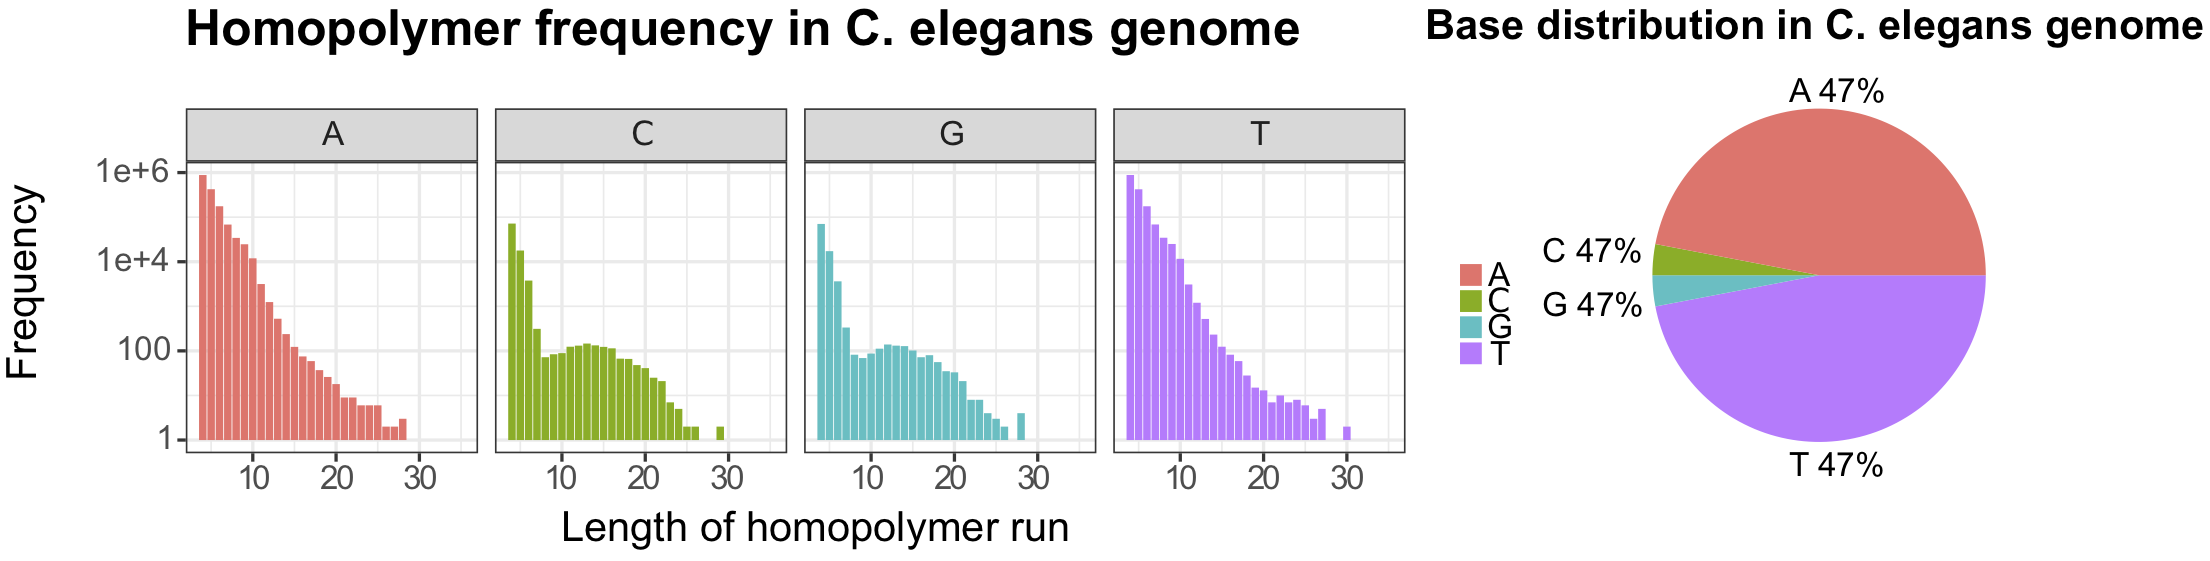
\includegraphics[width=1\textwidth]{figures/elegans_genome_homopolymers.png}}
  \caption{Distribution of homopolymeric sequences in \textit{C. elegans} genome.}
  \label{worm_homo}
\end{figure}


%%%%%%%%%%%%%%%%%%%%%%%%%%%%%%%%%%%%%%%%%%%%%%%%%%%%%%%%%%%%%%%%%%%%%%%%%%%%%%%%%%%%%%%%%%%%%%%%%%%

\section{Relation to replicationa and epigenetic features}

\subsection{Replication directionality}

\subsection{Localisation of mutations}

Microhomology, telomeres, clusters

\subsection{Epigenetic features}

\textbf{Incorporation of additional genetic information}. This includes validation of structural variants (namely, deletions and duplications) by analyzing copy number changes in the sample genomes, GC-content adjustment for correct comparison of substitutions types proportions, and removal of variants coming from low-complexity regions and highly repetitive regions. 

\textbf{Mitochondrial DNA} ????


%%%%%%%%%%%%%%%%%%%%%%%%%%%%%%%%%%%%%%%%%%%%%%%%%%

\section{Limitations of the analysis}

The current model concept does not account for several limitations coming from the nature of the data:
\begin{itemize}
\itemsep0em
\item Restricted number of mutations - some rearrangement can not be produced in sufficient number (negative selection)
\item Small number of replicates for each experiment (makes it hard to estimate the variance of the results)
\end{itemize}

\textbf{Overdispersion modeling}. The current data shows signs of significant overdispersion for most of the response classes: residual deviance (i.e. the difference in likelihood for the model under consideration versus saturated) is significantly greater than the residual degree of freedom.

This is probably due to the limitations mentioned earlier: in some cases there was not enough time to see any mutations, which does not allow us to extract the corresponding factor contribution. The presence of overdispersion makes the current estimates of coefficient standard errors biased, which leads to incorrect assessment of coefficients significance and reduced prediction variance (\cite{overdisp}).

In order to account for an excess of zero results, we will turn to Gamma-Poisson model (also known as negative-binomial model), setting a Gamma prior on the coefficients as in \cite{Ivek} and \cite{BNB}, which will help to correctly estimate the actual variance of the result and make better predictions.

\section{Discussion}

In this chapter, I described the concept of mutation accumulation experiments in \textit{C. elegans}, derived the mutational signatures of DNA repair deficiencies and genotoxins from a large screen, and provided insight into mechanistic background of these signatures.

The absence of effects for most of the genotypes studied indicates high level of redundancy among different DNA repair pathways, which means that it may require the combined deficiency of multiple DNA repair pathways to trigger excessive mutagenesis. Equally a latent defect in DNA replication integrity might only become apparent in conjunction with a DNA repair deficiency. Indeed the increased mutation burden detected in the \textit{pole-4}; \textit{pms-2} double mutant while no increased mutation rate is observed in \textit{pole-4} alone uncovered a latent role of \textit{pole-4}. It appears that replication errors occur at increased frequency in the absence of \textit{C. elegans} \textit{pole-4} but are effectively repaired by MMR.

*Genomic features*

*Some SV stuff*

*Talk about mutagens*

In the next chapter, I will exploit the means for cross-species comparison briefly introduced in this chapter, and show the usability of \textit{C. elegans} research to understanding the aetiology of mutations in human cancers.

%\newpage{}

%\appendix
%\section*{Appendix. Table of genetic knock-outs and mutagens used in the study with their interactions.}

%\begin{table}[h!]
%\centering
%\begin{adjustbox}{width=1\textwidth}
%\begin{tabular}{1.0*\textwidth}{|c|c|c|c|c|c|c|c|c|c|c|c|}
%\hline 
% & None & Aflatoxin & Cisplatin & DMS & EMS & HU & Mec & MMS & Rad & Xray & Pathway\tabularnewline
%\hline \hline
%N2 & allsubs, D, I, allSVs - INV  &  C$>$A & C$>$A, D & T$>$C, T$>$A, C$>$T, TD & allsubs, D  & C$>$T, C$>$A & D & allsubs – C$>$G, D, TD & allsubs, D & C$>$T, C$>$A, D, TD, INTCHR & \tabularnewline
%\hline 
%agt-1 & TD & & & & C$>$T, T$>$A & T$>$C, T$>$A, C$>$T &  &  &  &  & translesion synthesis	\tabularnewline
%\hline 
%\end{tabular}
%\label{app_table}
%\end{adjustbox}
%\end{table}

\end{document}